\documentclass[12pt]{article}
%Gummi|065|=)
\usepackage{amsmath, amsfonts, amssymb}
\usepackage[margin=0.5in]{geometry}
\usepackage{xcolor}
%\usepackage{graphicx}
%\usepackage{graphicx}
\newcommand{\off}[1]{}
\DeclareMathSizes{20}{30}{21}{18}

\newcommand{\myhrule}{}

\newcommand{\dash}{
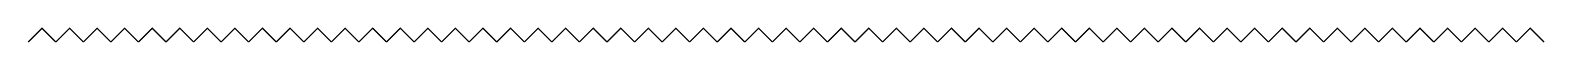
\begin{tikzpicture}[scale=0.35]
\foreach \x in {1,...,55}{
	\draw (\x,-0.25)--(\x+0.5,0.25)--(\x+1,-0.25);
}
\end{tikzpicture}
}

\usepackage{tikz}

\title{\textbf{ Examples: 2+1 Duality}}
\author{John D Mangual}
\date{}
\begin{document}

\fontfamily{qag}\selectfont \fontsize{25}{30}\selectfont

\maketitle

\fontfamily{qag}\selectfont \fontsize{12}{10}\selectfont

\noindent One very modern incarnation of the Fractional Quantum Hall effect is that of 2+1 dualities.\footnote{Encouraged by this year's Noble Prize in Physics, merely jumping into the 2016 literature here.  We can say something like this ``In attempting to learn FQHE and Chern-Simon's theory, I instead learned blah blah blah".  And off we go\dots}

\newpage

\fontfamily{qag}\selectfont \fontsize{12}{10}\selectfont

\begin{thebibliography}{}

\item Nathan Seiberg, T. Senthil, Chong Wang, Edward Witten. \textbf{A Duality Web in 2+1 Dimensions and Condensed Matter Physics} \texttt{arXiv:1606.01989}

\item Andreas Karch, David Tong
 \textbf{Particle-Vortex Duality from 3d Bosonization} \texttt{arXiv:1606.01893}

\item David Tong \textbf{Lectures on the Quantum Hall Effect} \texttt{arXiv:1606.06687}

\item Andreas Karch, Brandon Robinson, David Tong \textbf{More Abelian Dualities in 2+1 Dimensions} \texttt{arXiv:1609.04012}

\end{thebibliography}



\end{document}